\section{PDR2 processing on USDF cluster} \label{sec:processing}

The data processing was done using the Production and Distributed Analysis System (PanDA; \citeds{DMTN-168}) at the USDF at SLAC.
The PanDA system handled workflow orchestration and job retries.
Based on pre-production testing, five PanDA queues (\texttt{lowmem}, \texttt{mediummem}, \texttt{highmem}, \texttt{extra-highmem}, and  \texttt{merge}) were deployed. Each queue had fixed numbers of slots, memory limits, wallclock runtime limits and pull-or-push mode as described in this table:

The production processing was organized into seven logical ``steps''.
The high level workflow of workflows and the step organization is described in \citeds{RTN-001} Sect. 2.1.4.
Pipelines, V\&V, and Processing teams all focused on one step at a time.
Before the production processing started in each step, ``pilot runs'' with candidate software were carried out and signed off by V\&V and Pipelines teams
(Sect \ref{sec:management}).

The workflow generation and submission were done via the PanDA BPS plugin a terminal window logged into the USDF.
The BPS YAML configurations can be found in a branch of the  GitHub repo (https://github.com/lsst-dm/cm-prod).

Workflow progress was tracked via PanDA's iDDS monitoring page deployed at CERN and the JIRA-based campaign tooling (\citeds{RTN-023}).

On many occasions (20\%) rescue workflows skipping successful jobs were run.

The processing took place  between May 2023 to Sep 2023 and the total cpu usage over the course of PDR2 was approximately XXXX M core-hour; the compute resource usage is summarized below.
Notable issues which came up during the production were summarized as follows.

\begin{itemize}

\item Step1
\begin{itemize}

  \item
  The RSP’s ``large'' memory option has 12 GB and imposed a limit on the size (number of quanta) of the workflows that could be submitted, as otherwise quantum graph generation failed due to an out-of-memory error.
  A ``huge'' memory option became available in late January 2022, doubling the memory to 24 GB and enabling larger workflows to be submitted for subsequent processing steps.

  \item
  The quantum graph build time increased from about 1.5 hours for submissions at the beginning of step1 processing to about 8 hours at the end.
  This was due to the use of a single output chained collection, which needed to be examined in quantum graph generation, but which grew ever larger as production proceeded, thus increasing the graph generation time.
  To avoid this issue, starting in step3, we used separate output collections for the different workflow submissions in a given processing step, and then joined the separate collections together once all workflows were completed.

  \item
  To improve efficiency, we clustered together 315 quanta (consisting of different step1 tasks for multiple detectors in the same exposure) into a single job on the PanDA system.
  However, if one quantum failed among these 315 quanta, the whole job stopped and led to unattempted quanta.
  The intent for this behavior was so that downstream jobs would know about upstream failures, but in this case, the detectors were independent of each other, and there were no downstream jobs in our step1 workflows.
  To resolve this issue of unattempted quanta, we ran rescue workflows where quanta for different detectors were no longer clustered with each other.
  Subsequently the default behavior was changed so that an individual failure among clustered quanta would not stop the remaining quanta from being attempted.

\end{itemize} %step1

\item Step2
\begin{itemize}

 \item
 We expected that step2 would need a total of 3 workflows ($\approx$~6600 visits each), based on quantum graph generation tests, but execution butler creation became the bottleneck instead, and we instead required 14 smaller workflows ($\approx$~1500 visits each).
 For example, for the first of these smaller step2 workflows, quantum graph generation took 23 min, but execution butler creation took 7 hours, while job compute time was 2.5 hours (wall clock).
 Before step3 processing started, this issue was resolved in \jira{DM-33345}, and execution butler generation time was dramatically improved, e.g., from 7 hours down to 20 minutes in this step2 example, or from 1 hour down to 6.5 minutes for a 1-tract step3 workflow.

\end{itemize} %step2

\item Step3
\begin{itemize}

  \item
  Large numbers of simultaneous assembleCoadd (= image coaddition) jobs led to ``too many request'' errors reading from the object store (\jira{PREOPS-1034}).
  Algorithmically, the rate spike was because the coaddition was done in small chunks and data reading happened for each chunk and each input warp.
  This could be alleviated by caching input files instead of requesting them from the object store each time.
  The caching configuration in the butler repo was changed so not to expire anything in coaddition.
  The first 7 step3 workflows needed to be redone due to this problem.
  This also led to the investigation of the ``hidden'' errors in the coadds, where coadd images were reported ok but actually had problems (\jira{DM-33786}).
  More details are discussed in Sect. \ref{sec:qa}).
  Later we found out that the initial fix of the caching was too aggressive and led to out-of-disk-space errors for a couple of large faro tasks (matchCatalogsPatchMultiBand and matchCatalogsTract), but subsequently caching was better optimized to be sufficient for coadds, but not so much to cause disk space problems for the faro tasks.

  \item
  Long-running forcedPhotCoadd jobs were failing/re-attempting at a much higher rate than before, caused by a change in the PanDA pilot version, which reset the job heartbeat timeout limit back to its default of 2 hours, whereas it had been set to 20 hours previously.
  This issue also uncovered the need for more frequent heartbeat message logging for long-running forcedPhotCoadd (\jira{DM-33854}) and faro tasks (\jira{DM-33820}).
  The timeout limit was set again to 20 hours to allow step3 production to continue efficiently.

  \item
  About once every two workflows or so, a deblend job or two failed due to out-of-memory error (\jira{DM-33690}), because of very bright/large objects on the coadd image.
  These failures were fixed in rescue workflows, but required long run times ($>$10 hrs) and large memory ($\approx$~40 GB) using the \texttt{extra-highmem} queue, though ultimately with deblending results that were likely unreliable.
  The most extreme example (tract 4648, patch 29) took 12 unsuccessful attempts before finally succeeding in the \texttt{extra-highmem-non-preempt} queue (\jira{DM-33947}), after 2 days 22.7 hours run time, 190 GB memory, and extra efforts from the PanDA team to bypass heartbeat logging issues.
  This was the last image processing job to be completed in step3.
  \jira{DM-33690} implemented deblending configuration changes to skip these problematic deblends, so this should not be an issue subsequent to DP0.2.

  \item
  The large faro tasks matchCatalogsPatchMultiBand and especially matchCatalogsTract took long run times and large memory ($\approx$~130 GB for the latter).
  They needed to be run on the \texttt{extra-highmem} queue and were also prone to preemption and multiple re-attempts due to heartbeat logging issues (\jira{DM-33820)}.

 \item
  Some delays arose when jobs became stuck as they were unexpectedly scheduled to a non-IDF queue, which had its ``region'' set erroneously to ``LSST'', same as for the IDF queues.
  This issue was corrected by the PanDA support team.

  \item
  There were also some delays due to unexpected consequences from PanDA server and client updates, again resolved by the PanDA support team.

\end{itemize} %step3

\item Step4
\begin{itemize}

  \item
  An attempt was made to use the Google Artifact Registry (GAR) instead of Docker Hub to download the LSST processing stack.
  However, this resulted in intermittent authentication problems that led to 20-50\% job failures in three step4 workflows.
  Despite an attempt to reconfigure the IDF computing cluster involved, the authentication problems continued, and we reverted to using Docker Hub and reran the affected workflows.

  \item
  We also saw a drop in the maximum number of running jobs in the IDF queue involved, from nearly 4000 down to as few as about 2000, possibly related to the above authentication issues.
  PanDA support increased the maximum number of new worker nodes created from
50 to 80 to help stabilize the number of running jobs back to nearly 4000.


\end{itemize} %step4

\item step5
\begin{itemize}

  \item
  We encountered a very slow start to jobs running on the PanDA system due to the large number of jobs per task ($>$100,000) in the first step5 workflow.
  This was solved by reducing the maximum number of jobs per task from the default value of 70,000 down to 30,000, so that a single large task was divided into smaller ``chunks'' (each with $<$30,000 jobs) that ran much more efficiently in the PanDA system.
We do need an  iDDS server with more resources.

\end{itemize} %step5

\item step6, step7
\begin{itemize}

  \item Minor or no issues.

\end{itemize} %step6,7

\end{itemize} %all steps

 \begin{figure}
 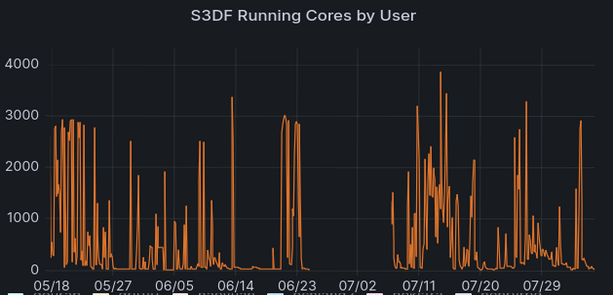
\includegraphics[width=0.9\textwidth]{Campcorespdr2.png}
         \caption{Cores in use in PDR2 step1,step2,step3 campaign.}  \label{fig:campaigncores}
 \end{figure}



